\documentclass[11pt, a4paper, oneside]{article}

\usepackage{indentfirst}

% hifenização e outras especificações para português
\usepackage[portuguese]{babel}

% hiperligações
\usepackage{hyperref}
\hypersetup{colorlinks=true, urlcolor=blue, linkcolor=black}

% escrever acentos e coisas do género sem que o latex se desoriente
\usepackage[utf8]{inputenc}

% para ter imagens, depois define a directoria de imagens
\usepackage{graphicx}
\graphicspath{{./imagens/}}

\usepackage[labelformat=simple]{caption}
\usepackage[labelformat=empty]{subcaption}

% para ter a informação de quantas páginas tem o documento
\usepackage{lastpage}

% definir o cabeçalho e rodapé
\usepackage{fancyhdr}
\pagestyle{fancy}
\fancyhead[L]{\small{Gestão de Campeonatos de Orientação}}
\fancyhead[R]{\small{Processamento de Linguagens}}

% ter enumerações alinhadas
\usepackage{enumitem}

% escrever algoritmos
\usepackage[algoruled]{algorithm2e}

% mais cores predefinidas
\usepackage[usenames,dvipsnames]{color}

% definir comandos especiais
\newcommand\doubleplus{+\kern-1.3ex+\kern0.8ex} %

\newcommand{\todo}[1] {\textcolor{BrickRed}{\begin{quote}#1\end{quote}}}

%\usepackage{listings}


%%%%%%%%%%%%%%%%%%%%%%%%%%%%%%%%%%%%%%%%%%%%%%
%% inicio do documento
\begin{document}
\title{Gestão de Campeonatos de Orientação}
\date{\today\\Universidade do Minho}
\author{
  Bruno Ferreira\\
  {\small A61055}\\
  \and
  Cláudia Oliveira\\
  {\small A60987}\\
  \and
  Vanessa Campos\\
  {\small A54801}\\
}

\maketitle

\begin{figure}[h]
\begin{center}

\includegraphics[width=0.4\linewidth]{logo}
\end{center}
\end{figure}


\begin{abstract}

  O presente trabalho foi desenvolvido no âmbito da Unidade Curricular de Processamento de Linguagens e tem como principal objetivo o aumento da experiência na Linguagem Imperativa C, a capacidade de escrever gramáticas independentes de contexto que satisfaçam a condição de LR(), a utilização de compiladores como o lex/yacc e o desenvolvimento de processadores de linguagem. Ao longo deste relatório iremos explicar as estruturas de dados que foram implementadas para o desenvolvimento deste trabalho, bem como todas as decisões que foram tomadas.

\end{abstract}
\newpage

\tableofcontents
\listoffigures 

\newpage
\section{Introdução}
A Orientação é um desporto que tem como objetivo percorrer uma determinada distância, onde o atleta tem de obrigatoriamente passar pelos pontos que estão indicados no mapa que lhe é atribuído.

Neste contexto temos a gestão de campeonatos de orientação onde é necessário saber a informação das provas que são efetuadas, os participantes envolvidos e os tempos que cada um obteve de modo a serem obtidas as classificações necessárias.
O objetivo principal é a leitura de ficheiros onde estes tem um configuração definida pelo ficheiro de configuração e depois a leitura do CSV com a informação dos jogadores e mais tarde o geramento de um página HTML onde é apresentada a informação tratada.

Para a implementação foi necessário a construção de gramáticas independentes de contexto, implementação de parses para cada ficheiro que necessário, e a utilização do lex e yacc para retirar a informação necessária.


\newpage
\section{Desenvolvimento}

\subsection{Contextualização do Problema}

Flex é uma ferramenta para gerar automaticamente analisadores léxicos, isto é, programas que reconhecem padrões léxicos num texto. O Flex é uma evolução da ferramenta Lex, mas com a caraterística de ser mais rápido que este (Fast Lex).

Yacc é utilizado para sistemas operacionais Unix, onde o seu principal objetivo e gerar analisadores sintáticos. No entanto o yacc tem de ser utilizado em conjunto com o lex, pois o yacc não consegue ler a partir de uma entrada de dados, daí a utilização  do lex para que este gere os tokens que mais tarde são usados pelo yacc para o processamento.

Gramática Independentes de contexto é uma gramática formal onde são definidas regras de produção da 
 V $\rightarrow$ W onde V é um símbolo não terminal e w um conjunto de símbolos terminais ou variáveis (W no entanto também pode ser nulo).

\subsection{Gestão de Campeonatos de Orientação }

Neste segundo trabalho de Processamento de Linguagens foi-no proposto a seleção de um projeto entre vários propostos. Após uma análise e chegada a uma concordância, o nosso grupo optou por escolher o tema de Gestão de Campeonato de Orientação.

Com este enunciado tem-se que existem várias operações que ocorrem em simultâneo, pois existe os ficheiros:
\begin{itemize}
\item Ficheiro de Resultados é um ficheiro CSV, onde são guardados os resultados obtidos em cada prova.

\item Ficheiro de Configuração é um ficheiro que vai definir o processamento a realizar, isto é quais as provas e os campos que vão ser tratados
\end{itemize}


\subsection{Enunciado}

De uma maneira geral, para este trabalho pretende-se desenvolver os seguintes pontos:

\begin{itemize}
\item Especificação de uma gramática para a linguagem de comandos da consola;
\item Especificação de uma gramática para a linguagem de especificação de connfigurações;
\item Especificação de uma gramática para os ficheiros de resultados;
\item Desenvolver os respetivos parses;
\item Adicionar as ações semânticas necessárias,
\end{itemize}


\subsection{Descrição do Problema}

Utilizando o flex, yac e gramáticas independentes de contexto era necessário a desenvolvimento de uma aplicação, que permita o tratamento de ficheiros e gere o HTML como os resultados pretendidos.

No entanto existem requisitos consoante ao funcionamento da aplicação. Esta deve possuir um ambiente de consola e implementar os seguintes comandos:
\begin{itemize}
\item Carregar configuração - Permite carregar o ficheiro de configuração;
\item Carregar base de dados - Carregar um ficheiro de dados previamente guardado;
\item Carregar resultado de prova - Carregar o ficheiro de resultados;
\item Calcular Ranking - Permnite calcular o ranking de pontuação dos atletas;
\item Gravar base de dados - Guardar a informação que existem na memória num ficheiro;
\item Sar -  Termina a aplicação.
\end{itemize}

É a partir daqui que os ficheiro de resultados e configuração são lidos e depois as operações são executadas. 

Antes de ser criado o HTML a aplicação tem de ser configurada.
A informação para tal é lida de um ficheiro de configuração onde nele são definidos os campos:
\begin{itemize}
\item Titulo - Titulo da prova em causa;
\item nporvas - nº de provas a realizar;
\item N - Indicados do topN ;
\item campos - Ordem dos campos quando no CSV;
\item score - Pontuação obtida;
\end{itemize}




\newpage

\subsection{Desenvolvimento do Programa}
Como este projeto implica muito o tratamento de de diferentes aspetos, foi decidido estruturar-se o projeto consoante as  funções que cada ficheiro implica.

\subsubsection{Estrutura de Dados}
Para a criação das estruturas de dados, foi usado a ferramenta \textit{gabs} disponibilizada pelo professor que cria a estrutura e os seus construtores quando é executada com uma gramática abstrata com argumento.

De modo a utiliza-se a ferramenta era necessário a criação de uma gramática abstrata que depois iria ser passada aos gabs.

Abaixo será apresentado um exemplo da implementação, no entanto em \ref{sec:Anexos} Anexos  puderam ser consultadas as restantes gramáticas abstratas.

A gramática a apresentar é a suada para o ficheiro de configuração. Assim sendo tem-se:
\begin{verbatim}
<ga>
  Confs -> cons_cfg_Confs(Conf Confs)
        |  cons_cfg_Confs_NIL()
        ;

  Conf -> cons_cfg_Conf_Titulo(STR)
       |  cons_cfg_Conf_Nprovas(INT)
       |  cons_cfg_Conf_Ntop(INT)
       |  cons_cfg_Conf_Campos(Lcampos)
       |  cons_cfg_Conf_Score(INT)
       ;

  Lcampos -> cons_cfg_Lcampos_Lcampos(Lcampos INT)
          |  cons_cfg_Lcampos_Campo(INT)
          ;
</ga>
\end{verbatim}

A estrutura que é gerada é:
\begin{verbatim}

struct sConfs 
{ int flag;
  union {  
    struct {
        Conf s1;
        Confs s2;
      } d1;
    struct {
      } d2;

  } u;
};


struct sConf 
{ int flag;
  union {  
    struct {
        char * s1;
      } d1;
    struct {
        int s1;
      } d2;
    struct {
        int s1;
      } d3;
    struct {
        Lcampos s1;
      } d4;
    struct {
        int s1;
      } d5;

  } u;
};


struct sLcampos 
{ int flag;
  union {  
    struct {
        Lcampos s1;
        int s2;
      } d1;
    struct {
        int s1;
      } d2;

  } u;
};
\end{verbatim}

Onde se tem que cada struct acima apresentada deriva de cada uma das produções que foram indicadas em na gramática abstrata.

\newpage

\section{Anexos}
\label{sec:Anexos}
\subsection{Gramáticas Abstratas}
\subsubsection{Gramática Abstrata Ficheiro Configuração}
\begin{verbatim}

\end{verbatim}

\subsubsection{Gramática Abstrata Ficheiro Comandos}
\begin{verbatim}

\end{verbatim}

\subsubsection{Gramática Abstrata Ficheiro CSV}
\begin{verbatim}

\end{verbatim}

\subsection{Estruturas de Dados}
\newpage
\section{Elementos do Grupo}
\begin{figure}[h!]
\centering
\begin{subfigure}{.33\textwidth}
  \centering
  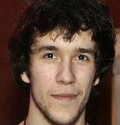
\includegraphics[width=0.8\linewidth]{60}
  \caption{Bruno Ferreira  }
\end{subfigure}%
\begin{subfigure}{.33\textwidth}
  \centering
  
\includegraphics[width=0.8\linewidth]{107}
  \caption{Cláudia Oliveira}
\end{subfigure}%
\begin{subfigure}{.33\textwidth}
  \centering
  
\includegraphics[width=0.8\linewidth]{93}
  \caption{Vanessa Campos}
\end{subfigure}%
\end{figure}


\end{document}